% Chapter Template

% Main chapter title
%\chapter[toc version]{doc version}
\chapter{Background}

% Short version of the title for the header
%\chaptermark{version for header}

% Chapter Label
% For referencing this chapter elsewhere, use \ref{ChapterTemplate}
\label{ChapterBackground}

% Write text in here
% Use \subsection and \subsubsection to organize text

This chapters main focus is to provide the reader with the necessary background information to understand the context of
this project. The main goal of this project is to provide a system capable of automatically evaluating network topologies 
by validating configurations and running tests on different devices in the network. Analogue systems exist in the market,
primarily focused in programming. These systems receive code from students and subsequently run tests on it against 
multiples test cases and are already widely deployed in educational environments. 
Shifting from programming to network topologies appears simple at first glance but comes with a particular set of 
challenges not present in programming evaluations. Each student will require an individual working environment, which can 
be addressed by using virtualization platforms. There is also the matter of communicating with the devices in the network, 
which can be addressed by using network automation tools. Finally there is the matter of combining these technologies to 
create a system capable of automatically evaluating network topologies.

\section{Programming Evaluation Systems}
While not directly related, they are the main inspiration for this project. Programming evaluation systems are widely
deployed in universities and other educational institutions. These systems receive code from students and subsequently run
tests on it, outputting a score and even being configurable to provide students the first test case that they failed in, 
guiding students to the solution without handing it out.

These tools typically provide a structured approach to test coding and problem solving skills. They begin by offering a
problem statement coupled with an optional image and an example test case, normally in the form of input and expected output.
Users can interact with the system by use of an online code editor, where they can write their solution and submit it for
evaluation, or by uploading a file with their solution. The system then evaluates the provided solution against multiple
pre-defined test cases, and validating the output against the know-good output, outputting a score based on the number of 
test cases passed. The system may also be configured to have time and/or memory constraints, to ensure that temporal and
spatial complexity are also taken into account.

All of these, serve to provide a thorough evaluation of the student's solution, which can help guide a student to better
their coding and problem solving skills.

In the context of the\ac{dcc}, Mooshak and Codex are commonly deployed to be used in the context of classes and 
even exams and programming contests.

The main differentiator between these systems and the one proposed in this project is the ability to solve a network 
exercise using multiple configurations across multiple devices, while programming evaluation systems will expect
the same output every time, given the same input.
Another key difference is the fact that programming evaluation systems dont always provide a working environment for the 
students to test their code, owing to the fact that students might prefer to user their own development environment for 
initial development and testing. This project aims to provide a working environment for students to work on for a few
reasons that will be discussed later on \unsure{DISCUSS REASONS WHY LATER}

\subsection{Mooshak}
Mooshak is a web-based system for managing programming contests and also to act as an automatic judge of programming 
contests \cite{Leal2003567}. It supports a variety of programming languages like Java, C, etc. Under each contest students will find one more 
problem definitions each containing varying sets of test cases in input-output pairs. After submiting their solution, 
the system will compile and run the code against the test cases giving a score based on the the amount of test cases passed.
The system can also differentiate between differing types of errors, such as not giving the expected output, poorly 
formatted output, failure to compile or even exceeding the time limits.
Mooshak also includes some features designed to drive competition between students, like a real time leaderboard and
the ability to have more than 100\% of the score for a given contest.

The system however is not without its limitations as it uses plain text files for its test cases and validates the output 
of student's code character by character, which can lead to false negatives if the output is not formatted exactly as
expected.

\section{Virtualization}
Virtualization is the process of creating a virtual version of physical resources, such as routers, switches, or even
entire computers. In the context of this project, it is used to create virtual machines to provide students with a 
work environment and virtual networks, comprised of various types of virtualized devices. This approach enhances scalability 
and reduces costs, as it allows multiple virtual machines to be run on a single physical machine.

Virtualization can be categorized into \textbf{emulation} and \textbf{simulation}. 

\begin{itemize}
  \item Emulation is the process of creating a virtual version of a physical device in software, replicating its 
  behavior exactly—including any bugs and limitations. This is useful for various things like testing software on 
  different platforms, running legacy software on modern hardware and even running potentially harmful software in a safe 
  isolated environment.
  Emulation will be used to provide students with a work environment to test their network configurations,
  as well as to emulate certain network devices.
  \item Simulation models the behaviour of a device, without replicating the underlying hardware or software.
  This results in a simpler less resource intensive model, though it may not fully capture the real device's behavior.
  Simulation will be used to simulate the behaviour of certain, simpler and generic, network devices.

\end{itemize}


\section{GNS3}
\ac{gns3} is an open-source graphical network emulator software that allows the user to create complex network topologies 
and interact with the various devices in it. It is widely used for educational purposes and is often used in preparation 
for professional network certifications like the Cisco Certified Network Associate (CCNA).

\ac{gns3} employs a simple drag and drop interface to allow users to add new devices, make links between them 
and even add textual annotations. The software allows users to interact with the devices by way of a console or even a GUI
if the device supports it. The software also allows users to export their topologies to be shared with others, which can
be useful for teachers to provide students with a pre-configured topology to work on.

Additionally, the software supports packet capturing which is essential for students to develop their debugging and 
troubleshoting skills. Finally it can also be interacted with via a\ac{rest}\ac{api} which is of particular interest
for this project.

\subsection{Architecture}
The software can be employed in a variety of ways due to its architecture \cite{GNS3Architecture} that separates the user 
interfaces that it offers, namely the locally installed gns3-gui as well as the browser accessible gns3-web, from the 
gns3-server that runs the emulations and the controller who orchestrates everything.

\subsubsection{Controller}
The controller is integrated in the gns3-server project and is responsible for communicating with all the other components 
of the software. The controller is a singleton, meaning there should only be one instance of it running at any given time, 
and it does not support concurrent requests. It is able to control multiple compute instances if so desired, each capable 
of hosting one or more emulator instances, varying depending on their complexity. The controller also exposes the 
\ac{rest}\ac{api} allowing the ability to interact with the software programatically. All communication is done over
\ac{http} in\ac{json} format and there is support for basic\ac{http} authentication as well as notifications via websockets.

\subsubsection{Compute}
The compute is also integrated in the gns3-server project and controls the various emulators required to run the nodes 
in the topology.
The list of currently supported emulators is:

\begin{itemize}
    \item \textbf{Dynamips} - Used to emulate Cisco routers and basic switching.
    \item \textbf{\ac{iou}} - Used to emulate Cisco\ac{ios} devices.
    \item \textbf{\ac{qemu}} - Used to emulate a wide variety of devices.
    \item \textbf{\ac{vpcs}} - A basic program meant to simulate a basic PC.
    \item \textbf{VMware/VirtualBox} - Used to run virtual machines with nested virtualization support.
    \item \textbf{Docker} - Used to run docker containers.
  \end{itemize}

\subsubsection{GUI}
The GUI is composed of two separate but with mostly identical functionality, namely the gns3-gui and the gns3-web projects.
The gns3-gui project is a desktop application that is used to to interact with a local or remote gns3-server instance. It 
is written in Python and uses the Qt framework for the graphical interface. The gns3-web is a web application that is 
accessed via a web browser it is still in a beta stage but is already capable enough to be used as a substitute for the 
gns3-gui.

\begin{figure}
    \centering
      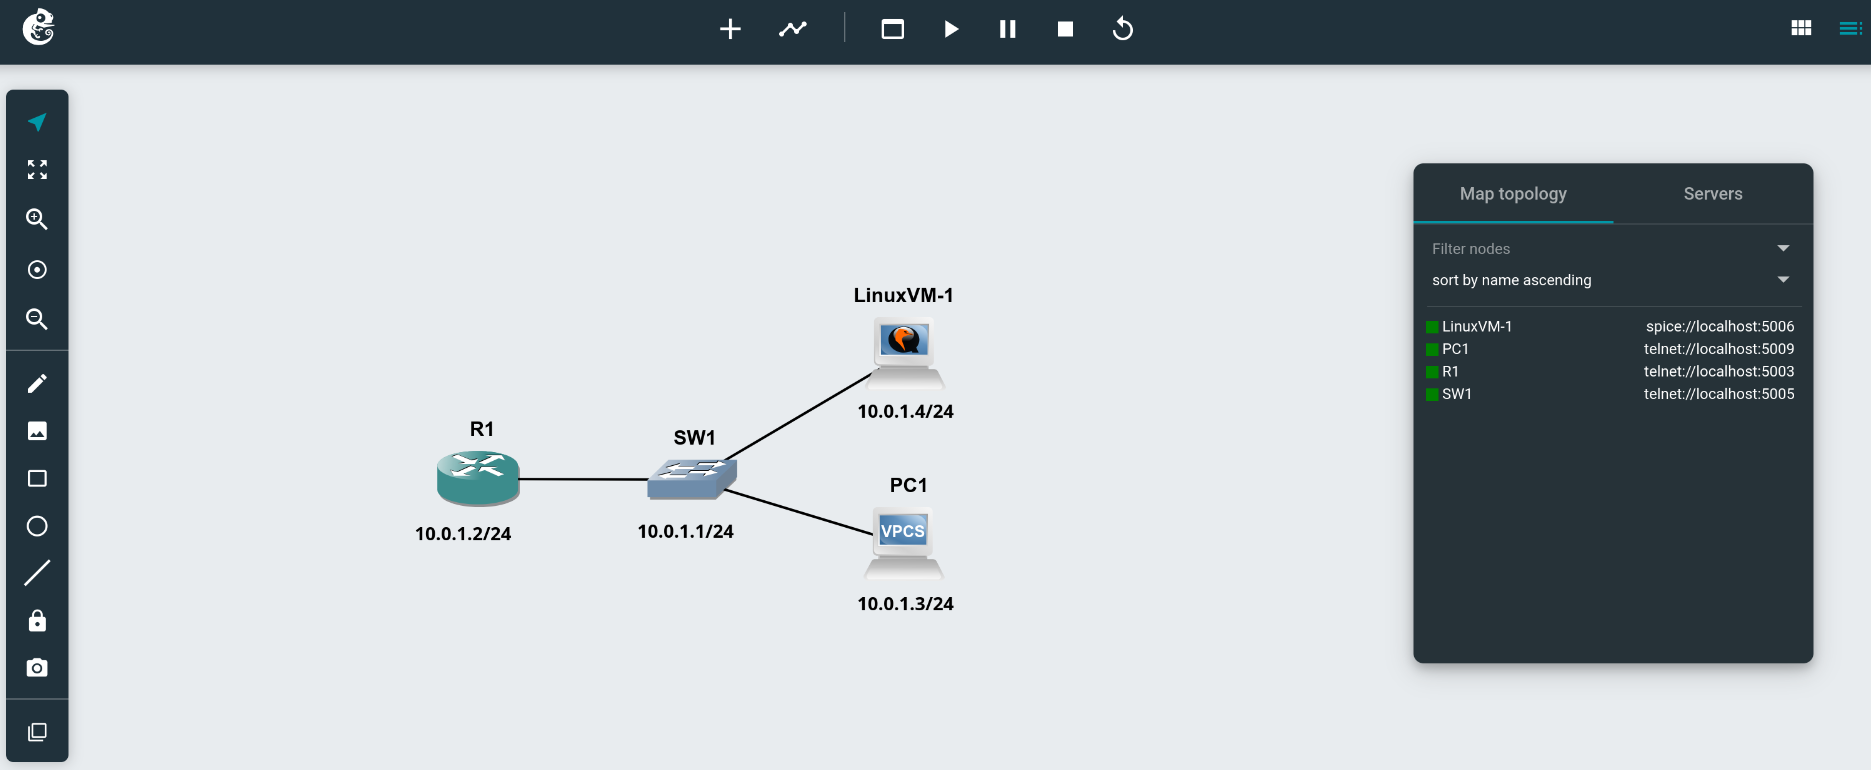
\includegraphics[width=.95\linewidth]
        {Background/gns3-web.png}
    \caption{A simple network topology example in the GNS3 Web UI}
	\hfill
\end{figure}

\section{Linux}
Linux is a core component of this project, as it is the operating system used to host all the services provided.

\begin{itemize}
  \item \textbf{Containerized Flask Application} \info{"Flask" subject to change} - The Flask web application runs inside 
  an LXC container on Proxmox. Since LXC containers share the host kernel, the containerized Flask app benefits from 
  efficient resource usage while maintaining isolation from the host system.
  \item \textbf{Virtual Machines hosting GNS3} Proxmox also hosts virtual machines running Linux-based Ubuntu GNS3 servers. 
  These VMs provide students with isolated environments to configure and test network topologies, benefiting from the 
  flexibility of full virtualization through KVM, giving them the ability to virtualize any type of network device.
  Students only interact with these \ac{vm}s via the GNS3 web Interface.
  \item \textbf{\ac{pve}} - Proxmox is a Linux-based open-source platform for enterprise-level virtualization. It is based
  on the Debian Linux distribution.
\end{itemize}


\section{Proxmox Virtual Environment} 
\ac{pve} is an open-source platform designed for enterprise-level virtualization \cite{proxmox2025}. It is based on the Debian
distribution of Linux and provides a web-based interface for managing virtual machines and containers. It is widely used
in data centers and cloud environments, as it provides a scalable and reliable solution for virtualization.

\ac{pve} bundles several core services that can be interacted with via shell commands, a web interface or even by using
the \ac{pve}\ac{rest}\ac{api}.
These allow the user to interact with every service provided by \ac{pve}, in a plethora of ways, depending on the user's
needs, skills and preferences. The web interface is the most user-friendly way to interact with the platform, as it
provides a graphical interface for managing the cluster. The shell commands provide a more direct way to interact with the
platform, allowing for more complex operations to be performed and opening the doors to scripting and automation. Finally,
the \ac{pve}\ac{rest}\ac{api} allows for programmatic interaction with the platform, enabling users to create custom
applications that can interact with the platform.


\subsection{Virtualization Technologies}
\ac{pve} supports the the deployment and management of two distinct types of virtualization, namely, \ac{kvm}- 
based\ac{vm}s and\ac{lxc}-based containers.

Users can interact with these virtualized environments via NoVNC, a simple web-based VNC client or SPICE which is a more
feature-rich protocol that provides better performance and more features than VNC.
Both of these protocols support the use of a console-based interface, aswell as a full desktop graphical interface.


\subsubsection{\ac{kvm}}
\ac{kvm} is a virtualization solution provided by the Linux kernel. It leverages the hardware virtualization extensions 
of modern processors to provide a full virtualization experience at near-native speeds. Supports a wide range of guest 
operating systems making it a good choice for general purpose virtualization.

In \ac{pve},\ac{kvm} is used as the core component for running virtual machines and is used alongside \ac{qemu}.

\subsubsection{\ac{lxc}}
Containerization is an operating system-level virtualization method that packages an application and its dependencies
together into an isolated environment. Contrary to tradional\ac{vm}s, containers dont emulate hardware or require a 
guest operating system relying instead on the host's kernel. This approach leads to a faster and more lightweight 
virtualization solution, as they consume less memory and cpu resources.

\ac{lxc} creates full system containers, capable of simulating a complete Linux distribution providing users with an 
environment that behaves like a traditional\ac{vm} but with the speed and efficiency of a container. \ac{lxc} start 
much faster than \ac{vm}s making them ideal for scenarios requiring rapid deployment and/or scaling.

However, it's important to note that while containers offer a degree of isolation, they do not provide the same level of
security as\ac{vm}s. This means that while they may not always be a suitable replacement for\ac{vm}s.

\section{Python}
Python is a high-level, interpreted programming language renowned for its readability and versatility. It supports 
multiple programming paradigms, including procedural, object-oriented, and functional programming, making it suitable 
for a wide array of applications.
In the context of this project, Python serves as the primary programming language as its extensive standard library 
and supportive community contribute to efficient development and maintenance of the project's codebase.

\section{WSGI}
The\ac{wsgi} is a pivotal standard for Python web application deployment, defining a consistent interface between web 
servers and Python applications or frameworks.

Prior to \ac{wsgi}'s introduction, Python web frameworks were typically written against various server-specific APIs such as 
CGI, FastCGI, or mod\_python. This diversity led to compatibility issues, limiting developers' choices of web servers and 
frameworks, as not all frameworks supported all web servers and vice-versa. To address this fragmentation, \ac{wsgi} was 
created as a standardized interface, promoting portability and flexibility in deploying Python web applications. 

\ac{wsgi} serves as a bridge, enabling web servers to communicate with Python applications. It specifies a simple and universal 
interface for web servers to forward requests to Python applications and for those applications to return responses. 
This standardization allows developers to choose from a variety of web servers and Python frameworks without compatibility 
concerns\cite{pep333}.

Introduced in 2003 as PEP 333, \ac{wsgi} was later updated to PEP 3333 in 2010 to accommodate Python 3. These specifications 
outline how web servers and Python applications should interact, ensuring a consistent and reliable deployment environment 
across different platforms.

The \ac{wsgi} standard consists of two main components:
\begin{itemize}
  \item \textbf{Server/Gateway Side} - Responsible for receiving\ac{http} requests from clients and passing them to the 
  Python application. Then receives the response from the application and forwards it to the client. 
  \item \textbf{Application} - The Python application that processes requests and returns responses.
\end{itemize}

Additionally \ac{wsgi} has support for middleware components. \ac{wsgi} middleware is a Python callable that wraps another 
\ac{wsgi} application to observe or modify its behavior. Middleware can perform various functions, including request 
preprocessing, response postprocessing, session management, and security checks. This modularity allows developers to 
add functionality to their applications in a reusable and maintainable manner.

The separation defined by \ac{wsgi} allows for flexibility and scalability in deploying Python web applications.

During development, Python web applications often use built-in servers provided by frameworks like Flask. 
However, these servers are not suitable for production environments. In production, WSGI servers act as intermediaries 
between web servers (e.g., NGINX or Apache) and Python applications, handling incoming requests and serving responses 
efficiently.

\subsection{Flask}
Flask is a web application micro framework written in Python, adhering to the \ac{wsgi} standard, designed to 
facilitate the development of web applications by providing essential tools and features. Classified as a microframework, 
Flask does not require particular tools or libraries, instead choosing to focus on simplicity and extensibility\cite{flask2025}.

Here, Flask serves as the backbone for the entire project, providing the necessary infrastructure to handle HTTP 
requests, render templates, and manage application routing. Its flexibility and minimalistic approach allow for the 
integration of various extensions and libraries as needed, ensuring the application remains lightweight yet functional. 
Flask's comprehensive documentation and supportive community further enhance its suitability by the creation and support
of community-driven extensions speeding up development and reducing the need to reinvent the wheel.
\unsure{flask might be changed to Quart of FastAPI}

An example of how easy it is to develop a basic web application with flask is provided in the following small 
piece of code.

\begin{algorithm}
  \caption{Flask Hello World}\label{flask-hello-world}
  \begin{algorithmic}[1]
    \State \textbf{from} flask \textbf{import} Flask
    \State \textbf{app} = Flask(\_\_name\_\_)
    \State
    \State \textbf{@app.route('/')}
    \State \textbf{def} hello\_world():
    \State \hspace{1em} \textbf{return} 'Hello, World!'
    \State
    \State \textbf{if} \_\_name\_\_ == '\_\_main\_\_':
    \State \hspace{1em} app.run()
  \end{algorithmic}
\end{algorithm}


\subsubsection{Asynchronicity}

\subsection{Nornir}
Nornir is an open-source automation framework written in Python, designed to provide a flexible and efficient 
approach to network automation tasks\cite{nornir2025}. Unlike other automation tools that utilize customized pseudo-languages, Nornir 
leverages pure Python code, offering developers the full power and versatility of the Python ecosystem.

Nornir supports multi-threaded task execution, allowing operations to run parallel across multiple devices.
This capability enhances efficiency and reduces the time required enabling easy scaling to a large number of devices.

The framework provides a robust inventory management system, enabling the organization of devices into groups and the 
assignment of specific tasks to these groups. This structure facilitates targeted automation and simplifies complex 
network operations.

Finally, thanks to nornir's architecture, it is highly extensible through its plugin system, allowing users to create 
custom plugins for inventory management, task execution, and result processing. This modularity ensures that Nornir can 
adapt to a wide range of network automation scenarios.

Nornir is particularly well-suited for tasks such as configuration management and state validation which makes it 
highly desirable in the context of this project. Its ability to handle concurrent operations will also ensure it can scale 
alongside the rest of the project.

\subsection{Requests}
The requests\cite{requests2025} library is a popular and user-friendly\ac{http} library for Python, used to send\ac{http} requests to web 
services. It simplifies interactions with APIs by simple to use methods for the various\ac{http} verbs, as well as
providing support for cookies, sessions, authentication, \ac{json} and exception handling for network failures and 
invalid responses.




\info{ Main technologies used to talk about
Python
Nornir
GNS3
ProxmoxVE
Flask -> quart/fastapi
Requests -> celery -> HTTPX
WSGI -> ASGI
Linux
NGINX?
Gunicorn?
}